%% This work may be distributed and/or modified under the
%% conditions of the LaTeX Project Public License, either version 1.3
%% of this license or (at your option) any later version.
%% The latest version of this license is in
%%   http://www.latex-project.org/lppl.txt



\documentclass[11pt,a5paper]{memoir}
\usepackage{ifxetex}

\usepackage{ifxetex}
\ifxetex
 \usepackage{polyglossia}
\setmainlanguage{brazil}
\setotherlanguages{french,english,spanish,german,italian}
\usepackage{fontspec}
\defaultfontfeatures{Ligatures=TeX}
\setmainfont{Minion Pro} %fonte principal (serifada)
\setsansfont{Myriad Pro} %fonte sem serifas
\setmonofont{Consolas} % fonte monoespaçada
 % comandos de fontes
\else
 \usepackage[utf8]{inputenc}
 \usepackage[T1]{fontenc}
 \usepackage{ebgaramond}
 % pacote de fontes
\fi


\usepackage[dvipsnames]{xcolor} % para cores
\usepackage{graphicx} % para imagens
\usepackage{booktabs} % para tabelas
\usepackage{lipsum} % para texto de preenchimento de exemplo
\usepackage{mdframed} % para caixas de texto como na CIP do verso do título
\usepackage{xspace} % para nao precisar de espaços com {} depios de comandos como \LaTeX e abreviações criadas pelo usuário
\usepackage[bookmarks,colorlinks]{hyperref}
\usepackage{microtype} %recomendável para melhorias de justificação
\usepackage[alf]{abntex2cite} %cuidado para colocar abntex2cite DEPOIS de hyperref!!!

\chapterstyle{veelo} % estilo de capítulo
\nouppercaseheads % para cabeçalhos sem estar em maiúsculas



\title{Exemplo de livro utilizando a classe ABN\TeX}
\author{Youssef Cherem}
\date{2013}

\begin{document}

\begin{titlingpage}

\phantom{xxx}
\vspace{0.5cm}
\huge
\raggedright
Fulano de Tal\\
\vspace{2.5cm}
\Huge 
{\raggedleft
\textit{\textcolor{red}{Exemplo de livro utilizando a classe}} ABN\TeX\\[1cm]
}
\centering 

\vfill
\Large
 Publicações Acadêmicas, Ltda.

\end{titlingpage}

\begin{titlingpage}

\phantom{xxx}
\vspace{0.5cm}
\huge
\raggedright
Fulano de Tal\\
\vspace{2.5cm}
\Huge 
{\raggedleft
\textit{\textcolor{red}{Exemplo de livro utilizando a classe}} ABN\TeX\\[1cm]
}
\centering 

\vfill
\Large
 Publicações Acadêmicas, Ltda.

\clearpage
\footnotesize
%\raggedright
© 2013 Fulano de Tal \& Publicações Acadêmicas, Ltda.
%este é só um exemplo de copyright.

Qualquer parte desta publicação pode ser reproduzida, desde que citada a fonte.

\bigskip

\begin{center}
Dados Internacionais de Catalogação na Publicação (\textsc{cip})
Câmara Brasileira do Livro, \textsc{sp}, Brasil
\end{center}

\begin{mdframed}
\noindent Tal, Fulano de.

Exemplo de livro utilizando a classe ABN\TeX. / Fulano de Tal. -- São Paulo: Publicações Acadêmicas, Ltda., 2013.

\medskip

Bibliografia.

ISBN XXXX-XXXX-XX.

\medskip

1. Programas de computador. 2. Tipografia. 3. Latex. 4. Normas ABNT.

\end{mdframed}

\end{titlingpage}



\frontmatter

\tableofcontents*
\cleardoublepage

\listoffigures*
\cleardoublepage

\listoftables*
\cleardoublepage

\mainmatter

\chapter*{Introdução}
Este documento destina-se a servir como modelo para composição e diagramação de livros em \LaTeX. Ele foi concebido para servir de base para elaboração de livros baseados na norma 6029 (de 2003) da \textsc{abnt}, para livros. A formatação de geral dos capítulos, margens, tamanho de página, fontes etc. pode ser modificada pelo usuário.


\chapter{Um exemplo de capítulo}

\chapter{Exemplos de imagens}

\begin{figure}
\centering
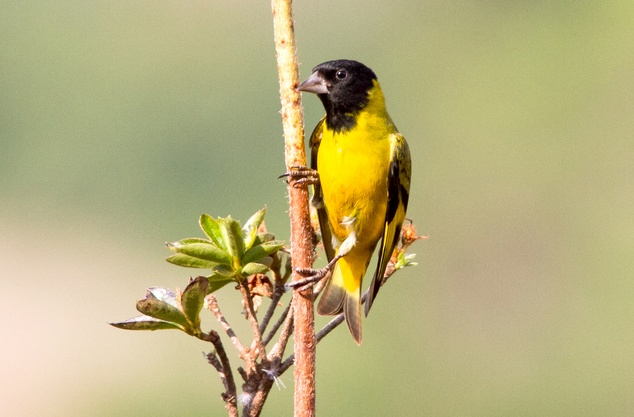
\includegraphics[width=0.6\linewidth]{pintassilgo}
\caption{Pintassilgo (\textit{Carduelis magellanicus}).}
\label{fig:pintassilgo}
\end{figure}


\begin{figure}
\centering
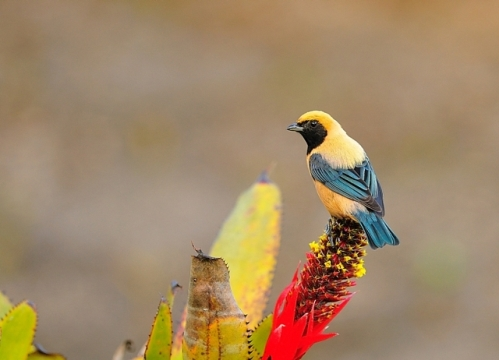
\includegraphics[width=0.6\linewidth]{saira-amarela}
\caption{Saíra-amarela (\textit{Tangara cayana}).}
\label{fig:saira-amarela}
\end{figure}

\begin{figure}
\centering
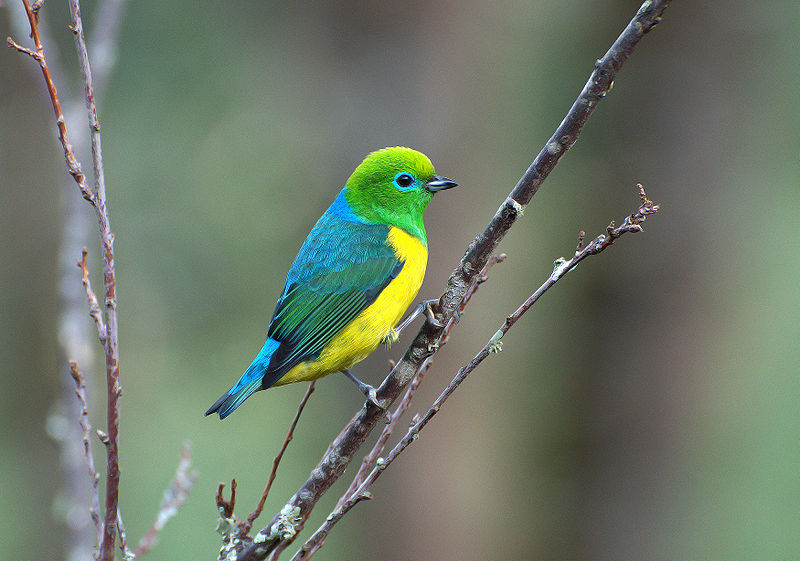
\includegraphics[width=0.6\linewidth]{bandeirinha}
\caption{Bandeirinha (\textit{Chlorophonia cyanea}).}
\label{fig:bandeirinha}
\end{figure}




\chapter{Um exemplo de capítulo}
\section{Um exemplo de tabela}
\begin{table}
\caption{Exemplo de tabela utilizando o pacote \textsf{booktabs}.}
\begin{tabular}{llr}
\toprule
\multicolumn{2}{c}{Item} \\
\cmidrule(r){1-2}
Animal    & Description & Price (\$) \\
\midrule
Gnat      & per gram    & 13.65      \\
          & each        & 0.01       \\
Gnu       & stuffed     & 92.50      \\
Emu       & stuffed     & 33.33      \\
Armadillo & frozen      & 8.99       \\
\bottomrule
\multicolumn{3}{l}{\footnotesize Fonte: \url{http://en.wikibooks.org/wiki/LaTeX/Tables}}
\end{tabular}
\end{table}

\chapter{Exemplos de citação}

Uma citação de Fulano: \citeonline{fulano}.

\cite{fulano}.


\bibliography{teste} % insere o arquivo de bibliografia (.bib)

\backmatter % pós-textual
\cleardoublepage
\thispagestyle{empty} % para última página com informações sobre a composição do livro.
~\vfill
Este texto foi composto em Minion Pro, de Robert Slimbach, e Myriad Pro, de Robert Slimbach e Carol Twombly.


\end{document}